\chapter{Der Transformer} \label{Transformer}

In der zweiten Hälfte des Jahres 2017 veröffentlichte ein Team von Wissenschaftlern ihr Papier \textquotedblright Attention Is All You Need\textquotedblright \cite{Vaswani:2017}, in welchem sie ein neues Modell vorstellten. Das Projekt zur Entwicklung wurde unter Google Research and Google Brain aufgeführt. Dieses Modell bekam den Namen "Transformer".

\section{Struktur des Transformers}
Der Transformer besteht aus zwei Haupteinheiten, deren Namen Encoder und Decoder sind \cite{Vaswani:2017}. Die beiden Einheiten bestehen aus gleicher Anzahl Encoder-, bzw. Decoder-Layers. Der im Artikel vorgestellte Encoder verfügte über 6 Encoderschichten und 6 Decoderschichten. Die \cref{transformer} beschreibt den Transformer.

In den linken Schichten fließt der Input, meistens mehrere Sätze, durch eine Attention- und eine FeedForward-Network(FFN)-Schicht. Rechts werden die Targeteingaben, die zugehörigen Sätze für den Input, von zwei Attention- und von einer FFN-Unterschichten bearbeitet. Der Input- und der Targetsatz werden eingebettet, bevor sie in den Encoder, bzw. Decoder, eingegeben werden. Nachdem der Einbettungsvektor steht, wird dieser durch eine positionelle Kodierung beeinflusst. Das erfolgt, indem der Positionsvektor mit dem Einbettungsvektor zusammenaddiert werden.

Die nächsten Unterkapitel betrachten die einzelnen Aufbauelemente des Transformers im Detail. Wichtig ist es, anzumerken, dass die positionelle Einbettung von keiner Einheit im Transformer berechnet wird, sondern die Ausgabe einer Funktion ist. Diese ist im nächsten Kapitel erläutert.

\begin{figure}[H]
	\centering
	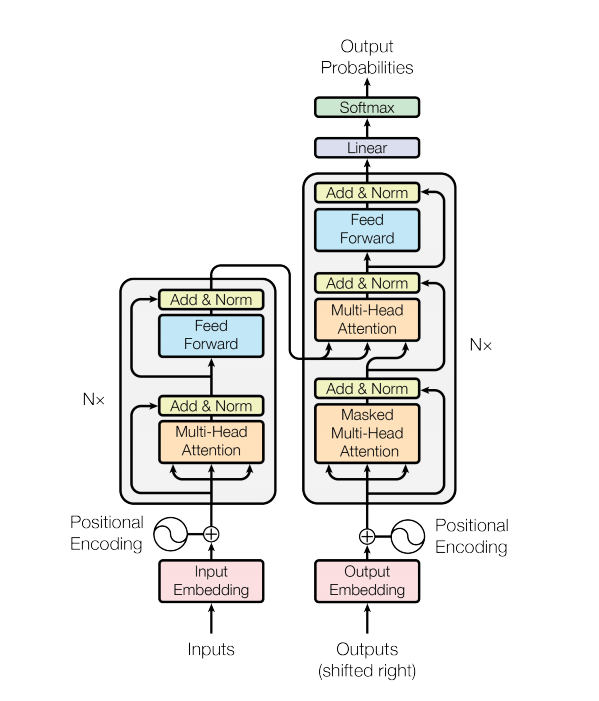
\includegraphics[scale=0.6]{images/transformer.png}
	\caption{Das Transformer-Modell \cite{Vaswani:2017}}
	\label{transformer}
\end{figure}

\subsection{Positionelle Einbettung}
Die positionelle Einbettung passiert nach der Umwandlung vom Text in Vektor. Wie die Bezeichnung verrät, wird Information über die Position des Wortes im Satz in den Wortvektor eingeschlossen. Diese zusätzliche Aktion ist eingesetzt, da der Transformer im Vergleich zu anderen Modellen oder Verfahren, kein Convolutional- oder Recurrent-Neural-Network beinhaltet.

Die Formel, nach der der Vektor berechnet wird, ist gegeben:

\begin{equation}
	PE_{(pos,2i)} = \sin\Bigg(\frac{pos}{10000^\frac{2i}{d_{model}}}\Bigg) \cite{denis_Transformer:02}
\end{equation}
\begin{equation}
	PE_{(pos,2i+1)} = \cos\Bigg(\frac{pos}{10000^\frac{2i}{d_{model}}}\Bigg) \cite{denis_Transformer:02}
\end{equation}

Der \textit{PE}-Vektor besteht aus $d_{model}$-Dimensionen, eine übliche Größe ist $d_model=512$. Für jede Dimension wird der Wert des Eintrages entweder mit der Sinus- oder Kosinusfunktion berechnet. Die geraden Dimensionen werden mit der Sinusfunktion und die Ungeraden mit der Kosinusfunktion kodiert.

Als nächstes wird betrachtet, wie der PE-Vektor im Einbettungs-Vektor eingelagert wird. In der Literatur werden die Vektoren ganz einfach addiert. Diese Vorgehensweise könnte jedoch Probleme verursachen und wichtige Informationen könnten verloren gehen. Es existieren mehrere Möglichkeiten, wie man den Verlust von Informationen vermeidet. In der Quelle \cite{denis_Transformer:02} wird folgende Formel benutzt:

\begin{equation}
	pc(i) = y_i*math.sqrt(d_{model}) + pe(i),
\end{equation}

wo der Eingabevektor $y_i$ durch eine Konstante $math.sqrt(d_{model})$ skaliert wird. Somit ist die Information aus der Einbettung verstärkt und der Einfluss des PE-Vektors vermindert. Die Variable $y_i$ ist der eingebettete Vektor, während $pe$ der Positionalsvektor und $d_{model}$ die Kardinalität eines Vektors ist. Der Eingabevektor wird mit der Wurzel von $d_{model}$ skaliert und erst dann wird der Positionalvektor addiert.

\subsection{Encoder und Decoder}

Encoder und Decoder sind die essenziellen Bestandteile des Transformers. Der Encoder erhält die Einbettung und führt sie durch ein Attention- und ein Feed Forward Network-Layer. Zwischen jeder Unterschicht besteht eine residierte Verbindung (siehe \cref{transformer}), sodass die Ausgaben von der letzten Unterschicht mit den Ausgaben von der Aktuellen addiert und weiterhin normiert werden. Der Decoder besitzt eine zusätzliche Unterschicht im Vergleich zum Encoder (\cref{transformer}). Im Transformer beihaltet der Decoder drei Schichten (siehe \cref{transformer}). Die letzten zwei sind die selben wie im Encoder. Die erste Teilschicht im Decoder ist eine Masked-Multi-Head-Attention-Schicht. Die Verbindung zwischen Encoder und Decoder erfolgt in der zweiten Unterschicht - nämlich in der MHA-Schicht. Da werden die Ausgaben vom Encoder und vom MMHA-Schicht zusammengeführt. Nach der Bearbeitung liefert das Model einen softmax-Vektor, der abhängig von der Aufgabenstellung die gesuchte Antwort sein sollte. In den folgenden Unterkapiteln werden die Unterschichten im Detail untersucht.

\subsubsection{Multi-Head-Attention Layer} \label{MHA_Layer}
Der Multi-Head-Attention Layer kommt in beiden Einheiten vor. Dieser Schicht folgt eine Masked-Multi-Head-Attention im Decoder und die Einbettungsschicht im Encoder.

Die Eingabe in dem Multi-Head-Attention-Layer vom Encoder ist der Vektor, der die positionellen und eingebetteten Angaben vom Text erhählt. Der Unterschied in der Schicht in Encoder und Decoder entsteht durch ihre Eingaben. Die Information ist für den Encoder komplett verfügbar, und im Decoder wird diese maskiert, und so lernt das Modell eine Prognose zu erstellen.

Ziel des MHA-Layer im Encoder ist es, die Beziehung zwischen einzelnen Wörtern zu bestimmen. Das wird erzielt, indem jedes Wort aus dem Satz mit allen anderen abgebildet wird. Das Problem dabei ist die Größe des Wortvektors, weil er eine Kardinalität von $d_{model}$ besitzt. In der Quelle \cite{denis_Transformer:02} erhält $d_{model}$ den Wert von 512. Die große Anzahl der Dimensionen würde große Laufzeit anfordern, wenn mehrere Ansichten untersucht werden. Das bedeutet wiederum, dass mehr Leistung erfordert wird, um weitere Ansichten zu bestimmen. Eine bessere Alternative ist es, die Dimensionen jedes Wortes, bzw. Satzes, in 8 Teile zu zerlegen, dabei besteht jeder Teil aus 64 Dimensionen. In \cite{denis_Transformer:02} ist jeder Teil als Head bezeichnet, daraus entsteht auch der Name \textbf{Multi-Head}-Attention-Layer.

\begin{figure}[H]
	\centering
	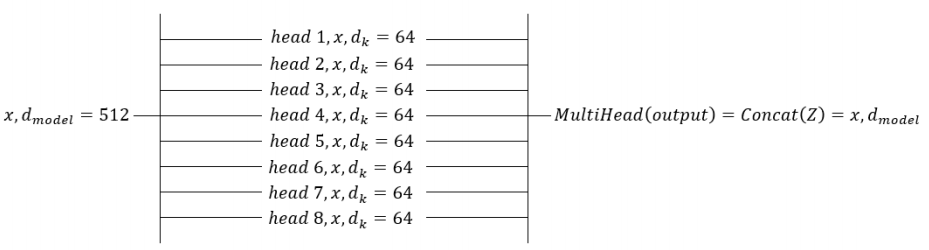
\includegraphics[scale=0.45]{images/multi_head.png}
	\caption{Heads \cite{denis_Transformer:02}}
	\label{multi_head}
\end{figure}

Diese Heads laufen parallel. Der Vorteil dabei ist es, dass die Laufzeit verringert wird und 8 unterschiedliche Repräsentationen betrachtet werden. In der \cref{multi_head} ist es zu erkennen, wie die MHA-Schicht aussieht. Nachdem die Daten von jedem Kopf vorhanden sind, werden die Ergebnisvektoren wieder konkateniert (siehe Abbildung \ref{multi_head}). Die Ausgabe sieht dann wie folgt aus:

\begin{equation}
	Z = (z_0, z_1, z_2, z_3, z_4, z_5, z_6, z_7) \cite{denis_Transformer:02}
\end{equation}

Die Matrix Z ist die aus den Ausgaben $z_i$ aufgebaute Ergebnismatrix. Am Ende muss die Matrix $Z$ zusätzlich konkateniert werden, um die ursprünglichen Dimensionen $x*d_{model}$ zu erhalten.

In jedem Kopf wird jedes Wort mit drei Vektoren repräsentiert \cite{transfered_learning:22}:
\begin{itemize}
	\item Einem Query-Vektor ($Q$), dessen Dimensionalität $d_q$ gleich \textbf{64} ist. Der Vektor wird verwendet, oder trainiert, wenn der zugehörige Wortvektor für $x_n$ die Key-Value-Paare der anderen Wortvektoren sucht, inklusive sich selbst bei Selbstattention.
	
	\item Einem Schlüsselvektor (auch als Key-Vektor bezeichnet $K$), der mit dem Ziel angepasst wird, einen Attention-Wert zu liefern.
	
	\item Einem Wertvektor (auch als Value-Vektor bezeichnet $V$), der darauft trainiert wird, einen weiteren Anttention-Wert bereitzustellen.
\end{itemize}

Die Quelle \cite{denis_Transformer:02} bezeichnet die Attention als \text{\quotedblbase}Scaled Dot-Product Attentionvon. Das ist eine Linearkombination der oben deklarierten Vektoren. Die folgende Formel aus \cite{denis_Transformer:02} stellt die Berechnung dar: 

\begin{equation}
	Attention(Q, K, V) = softmax\Bigg(\frac{Q*K^T}{\sqrt{d_k}}\Bigg)* V
\end{equation}

Diese Vektorrepräsentationen werden aus den Gewichtsmatrizen eingelesen. Die Gewichtsmatrizen sind am Anfang nicht bekannt und werden im Folge des Trainings bestimmt. Zu Beginn werden sie mit zufälligen Werten erstellt. Die Matrizen werden im Buch \cite{denis_Transformer:02} als $Q_w$, $K_w$ und $V_k$ beschriftet. Sie besitzen $d_k$ = \textbf{64} Spalten und $d_model$ = \textbf{512} Zeilen. Wenn zum Beispiel ein bestimmtes Query für das Wort $x_n$ abzulesen ist, dann erfolgt das durch eine einfache Matrixmultiplikation, wobei $x_n$ in diesem Fall den Indexwert vom Wort $x_n$ repräsentiert:
\begin{subequations}
\begin{equation}
	Q_{x_n} = x_n * Q_w
\end{equation}
\begin{equation}
	K_{x_n} = x_n * K_w
\end{equation}
\begin{equation}
	V_{x_n} = x_n * V_w
\end{equation}
\end{subequations}
Wenn die Eingabe aus mehreren Wörtern besteht, wird eine Matrix mit den Dimensionen \textit{Anzahl der Wörtern}$\times d_{model}$ (für $d_{model}$ meistens 512 gewählt) erhalten.

Für jeden Eintrag in \textit{x} wird eine Matrix mit ihren Attention-Vektoren, bzw. den Beziehungsvektoren zu jedem Eingabewort $x_n$ (inklusive sich selbst) berechnet. Jeder Vektor in der Matrix hat 512 Einträge, und es gibt insgesamt $m$-viele Vektoren ($m-viele$ Wörter). Der Attention-Vektor für jedes Wort wird erhalten, indem die Vektoren aus der Matrix summiert werden. Schließlich wird jedes Attention-Vektor von allen Heads zusammengeführt, und diese bauen die Attention-Matrix auf. Eine Normierungsschicht folgt der Attention-Schicht. Diese bekommt als Eingabe die konkatenierte Ausgabe von Matrix $Z_{concat}$ und die unveränderten Eingabedaten der MHA-Attentionschicht $x$:

\begin{equation}
	v = x + Z_{concat}.
\end{equation}
Mittels der Normierungsschicht werden dann folgende Berechnungen ausgeführt:

\begin{equation}
	LayerNorm(v) = \gamma * \frac{v - \mu}{\delta} + \beta. \cite{denis_Transformer:02}
\end{equation}
Die Variablen bedeuten Folgendes:

\begin{itemize}[leftmargin=1cm]
		\item $\mu$ ist der Durchschnitt von $v$ mit Dimensionen d:
		\begin{equation}
			\mu = \frac{1}{d}\sum_{k=1}^{d} v_k. \cite{denis_Transformer:02}
		\end{equation}
		\item $\delta$ ist die Standardabweichung von $v$ mit Dimensionen \textit{d}:
		\begin{equation}
			\delta^2 = \frac{1}{d}\sum_{d}^{k=1} (v_k - \mu)^2. \cite{denis_Transformer:02}
		\end{equation}
		\item $\gamma$ ist ein Skalierungsparameter.
		\item $\beta$ ist ein Bias-Vektor.
\end{itemize}

Die weiteren Normierungsschichten im Modell führen analoge Operationen und diese Erläuterung dient als Muster für die weiteren. Somit werden alle anderen Normierungsschichten nicht betrachtet.

Gleichermaßen sieht die Funktionalität der MHA-Schicht im Decoder aus. Die Eingabe in der Schicht besteht aus dem Masked-Multi-Head-Attention-Layer und der Ausgabe des Encoders. Als Nächstes wird der Feed-Forward-Network-Sublayer erläutert.

\subsubsection{Feed-Forward-Network}

Die Eingabe im Feed-Forward-Network ist die Ausgabe der Normierungsschicht (siehe Abbildung \ref{transformer}). Die Eingabe ist ein $d_{model}$ Dimensionales Vektor. Die Struktur des FFN-Layers kann wie folgt beschrieben werden \cite{Vaswani:2017}:

\begin{itemize}[leftmargin=1cm]
	\item Die Schichten sind sowohl im Encoder als auch im Decoder komplett verbunden.
	
	\item Die FFN ist für jedes Wort einzeln anzuwenden. Die Anwendung ist identisch, jedoch mit unterschiedlichen Parametern.
	
	\item Das Netzwerk besteht aus zwei Lineartransformationen und eine ReLU-Aktivierung dazwischen:
	\begin{equation}
		FFN(x) = max(0, x*W_1 + b_1)*W_2 + b_2.
	\end{equation}
	
	\item Die Ein- und Ausgabe des FFN haben eine Dimensionalität von $d_model$ = 512. Die innere Schicht besteht aus $d_{ff}$	= 2048 Neuronen.
\end{itemize}

Sowohl im Encoder als auch im Decoder ist die Struktur und Funktionalität der FFN-Schicht übereinstimmend. Die Ausgaben der FFN-Schicht werden wieder normiert. Die Inputdaten von der nachfolgenden Normierungsschicht sind die Ausgabe vom FFN und dessen Eingabe (in beiden Einheiten gleich; siehe Abbildung \ref{transformer}).


\subsubsection{Masked-Multi-Head Attention Layer}

Die letzte Schicht vom Decoder ist die Masked-Multi-Head-Attentnion-Schicht. Diese Schicht hat den gleichen Aufbau wie die MHA-Schicht. Diese Schicht unterscheidet sich von dieser im Encoder darin, dass die Eingabe  ``maskiert'' wird. Das bedeutet, dass bestimmte Abschnitte ausgeblendet werden, sodass der Layer begrenzte Informationen erhält. Ziel der Maskierung ist es, das Modell zu zwingen, die unbekannten Stellen zu raten. Deswegen betrachtet das Netz die Information nur bis zur aktuellen Position und die nachfolgenden Stellen müssen erraten werden.
%TODO:HIer den Satz überprüfen
\section{Implementierung}

Die Implementierung des Transformers ist sehr komplex. Der Programmcode kann außerdem auf der Tensorflow Seite \cite{transformer_tensorflow:21} gefunden werden. 

\subsubsection{Die Klasse}
Für den Aufbau des Modells werden 6 Klassen gebraucht. Diese sechs Klassen beschreiben die wichtigsten Komponenten des Transformers und das Modell selbst. Es gibt zwei Klassen für den Encoder und Decoder, zwei für die Layers im Encoder und Decoder, die Klasse für das Modell und eine Klasse für den Attentionlayer. Für einen besseren Überblick wird hier die Hauptklasse des Transformers vorgestellt:

\begin{lstlisting}[language=Python, caption={Definition des Transformers}]
self.encoder = Encoder(num_layers, d_model, num_heads, dff, input_vocab_size, pe_input, rate)
self.decoder = Decoder(num_layers, d_model, num_heads, dff, target_vocab_size, pe_target)
self.dense = Dense(target_vocab_size)
\end{lstlisting}

Die Codezeilen sprechen für sich. Die Dense-Schicht repräsentiert ein komplett verbundenes Netzwerk mit \textit{target\_vocab\_size}-vielen Neuronen. Die Ausgabe davon stellt die Prognose des Modells dar. Für jedes einzelne Wort im Satz wird der Decoded-Vektor in einen anderen Vektor mit Dimensionalität \textit{sequence\_length} $\times$ \textit{target\_vocab\_size} umgewandelt. Für jede Stelle im Satz liefert die Dense-Schicht einen Vektor, der so groß ist wie die Anzahl der einzigartigen Wörter im Targetcorpus. Jeder Eintrag in diesem Vektor stellt die Wahrscheinlichkeiten dar, dass das Wort an der Stelle platziert werden soll. Somit ratet das Modell. Der Encoder und Decoder werden mit den bestimmten Hyperparametern initialisiert. Im beschriebenen Fall wird ein Transformer mit folgenden Hyperparametern verwendet:

\begin{lstlisting}[language=Python, caption={Hyperparameter}]
num_layers = 6
d_model = 512
dff = 2048
num_heads = 8
\end{lstlisting}

Diese Variablen haben die gleiche Werte wie der ursprüngliche Transformer \cite{Vaswani:2017}.

\subsubsection{Encoder}

Die Encoder Klasse besteht aus mehreren Encoder-Schichten und aus der entsprechenden Embedding-Schicht. Die Klasse sieht wie folgt aus:

\begin{lstlisting}[language=Python, caption={Encoder}, label={Transformer_Enc_class}]
self.embedding = Embedding(input_vocab_size, d_model)
self.pos_encoding = self.positional_encoding(maximum_position_encoding, self.d_model)
self.enc_layers = [EncoderLayer(d_model, num_heads, dff, rate) for _ in range(self.num_layers)]
self.dropout = Dropout(rate)
\end{lstlisting}

Hier erkennt man die zwei Einbettungsschichten, eine für die Worteinbettung und die zweite für die positionelle Einbettung. In der dritte Zeile werden alle Encoderschichten erstellt. Am Ende wird eine Dropout-Schicht angehängt, die dabei Hilft, dass das Modell nicht übertrainiert (overfitted) wird.

\subsubsection{Decoder}

Die Decoder-Klasse wird ebenso in einer separaten Klasse ausgelagert. Die Programmzeilen \ref{trans_dec} widerspiegeln die vorgestellte Struktur des Decoders im oberen Kapitel \ref{transformer}: 

\begin{lstlisting}[language=Python, caption={Decoder Implementation}, label=trans_dec]
self.embedding = Embedding(target_vocab_size, d_model)
self.pos_encoding = self.positional_encoding(maximum_position_encoding, d_model)
self.dec_layers = [DecoderLayer(d_model, num_heads, dff, rate) for _ in range(num_layers)]
\end{lstlisting}

In der Zeile 3 aus dem \cref{trans_dec} werden die Decoder-Schichten erstellt. Ebenso werden in den Zeilen 1 und 2 die zwei Einbettungsoperationen für die Einbettungsschicht definiert. Die Embedding-Schicht unterscheidet sich von der Einbettungsschichten im Encoder, im Sinne von Variablen, und spielt die Rolle einer Look-up-Tabelle für das Targetcorpus.

